\documentclass{wissdoc}

% Autor: Roland Bless 1996-2009, bless <at> kit.edu
% ----------------------------------------------------------------
% Diplomarbeit - Hauptdokument
% ----------------------------------------------------------------
%%
%% $Id: diplarb.tex 53 2009-12-10 12:23:37Z bless $
%%
% wissdoc Optionen: draft, relaxed, pdf --> siehe wissdoc.cls
% ------------------------------------------------------------------
% Weitere packages: (Dokumentation dazu durch "latex <package>.dtx")
%\usepackage{bibgerm}
%\usepackage[backend=biber]{biblatex} 
\usepackage{csquotes} 
\usepackage{tabularx}
\usepackage{booktabs}
\usepackage{multirow}
%\usepackage{tocbibind}
\usepackage{siunitx}
\usepackage{xcolor}
\usepackage{textcomp}
\usepackage{listings}
\usepackage{newfloat,caption}
\usepackage{subcaption}
\usepackage{footnote}
\usepackage{rotating}
\usepackage{pgfplots}
\usepackage{pgfplotstable}
\usepackage{url}
\usepackage{boxhandler}
\usepackage{tabu}
\usepackage{amssymb}
%\usepackage{subfig}
%\usepackage{subcaption}
\usepackage{caption}
\usepackage{subcaption}
%\usepackage[plainpages=true]{hyperref}
\usepackage[space]{grffile}
%\usepackage[numbers,sort&compress]{natbib}
\usepackage[backend=bibtex,natbib=true,hyperref=true,doi=false,url=false]{biblatex}
%\usepackage{biblatex}
% \usepackage{varioref}
% \usepackage{verbatim}
\usepackage{float}    %z.B. \floatstyle{ruled}\restylefloat{figure}
%\usepackage[hidelinks]{hyperref}
% \usepackage{subfigure}
% \usepackage{fancybox} % für schattierte,ovale Boxen etc.
% \usepackage{tabularx} % automatische Spaltenbreite
% \usepackage{supertab} % mehrseitige Tabellen
% \usepackage[svnon,svnfoot]{svnver} % SVN Versionsinformation 
%% ---------------- end of usepackages -------------

%\svnversion{$Id: diplarb.tex 53 2009-12-10 12:23:37Z bless $} % In case that you want to include version information in the footer
%\hyphenation{if...-then...}
%% Informationen für die PDF-Datei
\pgfplotsset{compat=newest}

\hypersetup{
%%% styling of link inside pdf
	colorlinks,
  citecolor=black,
  filecolor=black,
  linkcolor=black,
  urlcolor=black,
%%%		
 pdfauthor={Sachin Rajgopal},
 pdftitle={Accessible EPUB}
 pdfsubject={Not set},
 pdfkeywords={Not set}
}
\DeclareFloatingEnvironment[fileext=frm,placement={!ht},name=Listing,within=section]{listing}

% Macros, nicht unbedingt notwendig
%%%%%%%%%%%%%%%%%%%%%%%%%%%%%%%%%%%%%%%%%%%%%%%%%%%%%%%%%%
% macros.tex -- einige mehr oder weniger nuetzliche Makros
% Autor: Roland Bless 1998
%%%%%%%%%%%%%%%%%%%%%%%%%%%%%%%%%%%%%%%%%%%%%%%%%%%%%%%%%%
% $Id: macros.tex 33 2007-01-23 09:00:59Z bless $
%%%%%%%%%%%%%%%%%%%%%%%%%%%%%%%%%%%%%%%%%%%%%%%%%%%%%%%%%%


%%%%%%%%%%%%%%%%%%%%%%%
% Kommentare 
%%%%%%%%%%%%%%%%%%%%%%%
\ifnotdraftelse{
\newcommand{\Kommentar}[1]{}
}{\newcommand{\Kommentar}[1]{{\em #1}}}
% Alles innerhalb von \Hide{} oder \ignore{} 
% wird von LaTeX komplett ignoriert (wie ein Kommentar)
\newcommand{\Hide}[1]{}
\let\ignore\Hide

%%%%%%%%%%%%%%%%%%%%%%%%%
% Leere Seite ohne Seitennummer, wird aber gezaehlt
%%%%%%%%%%%%%%%%%%%%%%%%%

\newcommand{\leereseite}{% Leerseite ohne Seitennummer, nächste Seite rechts (wenn 2-seitig)
 \clearpage{\pagestyle{empty}\cleardoublepage}
}
%%%%%%%%%%%%%%%%%%%%%%%%%%
% Flattersatz rechts und Silbentrennung, Leerraum nach rechts maximal 1cm
%%%%%%%%%%%%%%%%%%%%%%%%%%
\makeatletter
\newcommand{\myraggedright}{%
 \let\\\@centercr\@rightskip 0pt plus 1cm
 \rightskip\@rightskip
  \leftskip\z@skip
  \parindent\z@
  \spaceskip=.3333em
  \xspaceskip=.5em}
\makeatother

\makeatletter
\newcommand{\mynewline}{%
 \@centercr\@rightskip 0pt plus 1cm
}
\makeatother


%%%%%%%%%%%%%%%%%%%%%%%%%%
% Für Index
%%%%%%%%%%%%%%%%%%%%%%%%%%
\makeatletter
\def\mydotfill{\leavevmode\xleaders\hb@xt@ .44em{\hss.\hss}\hfill\kern\z@}
\makeatother
\def\bold#1{{\bfseries #1}}
\newbox\dbox \setbox\dbox=\hbox to .4em{\hss.\hss} % dot box for leaders
\newskip\rrskipb \rrskipb=.5em plus3em % ragged right space before break
\newskip\rrskipa \rrskipa=-.17em plus -3em minus.11em % ditto, after
\newskip\rlskipa \rlskipa=0pt plus3em % ragged left space after break
\newskip\rlskipb \rlskipb=.33em plus-3em minus.11em % ragged left before break
\newskip\lskip \lskip=3.3\wd\dbox plus1fil minus.3\wd\dbox % for leaders
\newskip \lskipa \lskipa=-2.67em plus -3em minus.11em %after leaders
\mathchardef\rlpen=1000 \mathchardef\leadpen=600
\def\rrspace{\nobreak\hskip\rrskipb\penalty0\hskip\rrskipa}
\def\rlspace{\penalty\rlpen\hskip\rlskipb\vadjust{}\nobreak\hskip\rlskipa}
\let\indexbreak\rlspace
\def\raggedurl{\penalty10000 \hskip.5em plus15em \penalty0 \hskip-.17em plus-15em minus.11em}
\def\raggeditems{\nobreak\hskip\rrskipb \penalty\leadpen \hskip\rrskipa %
\vadjust{}\nobreak\leaders\copy\dbox\hskip\lskip %
\kern3em \penalty\leadpen \hskip\lskipa %
\vadjust{}\nobreak\hskip\rlskipa}
\renewcommand*\see[2]{\rlspace\emph{\seename}~#1} % from makeidx.sty

%%%%%%%%%%%%%%%%%%%%%%%%%%
% Neue Seite rechts, leere linke Seite ohne Headings
%%%%%%%%%%%%%%%%%%%%%%%%%%
\newcommand{\xcleardoublepage}
{{\pagestyle{empty}\cleardoublepage}}

%%%%%%%%%%%%%%%%%%%%%%%%%%
% Tabellenspaltentypen (benoetigt colortbl)
%%%%%%%%%%%%%%%%%%%%%%%%%%
\newcommand{\PBS}[1]{\let\temp=\\#1\let\\=\temp}
\newcolumntype{y}{>{\PBS{\raggedright\hspace{0pt}}}p{1.35cm}}
\newcolumntype{z}{>{\PBS{\raggedright\hspace{0pt}}}p{2.5cm}}
\newcolumntype{q}{>{\PBS{\raggedright\hspace{0pt}}}p{6.5cm}}
\newcolumntype{g}{>{\columncolor[gray]{0.8}}c} % Grau
\newcolumntype{G}{>{\columncolor[gray]{0.9}}c} % helleres Grau

%%%%%%%%%%%%%%%%%%%%%%%%%%
% Anführungszeichen oben und unten
%%%%%%%%%%%%%%%%%%%%%%%%%%
\newcommand{\anf}[1]{"`{#1}"'}

%%%%%%%%%%%%%%%%%%%%%%%%%%
% Tiefstellen von Text
%%%%%%%%%%%%%%%%%%%%%%%%%%
% S\tl{0} setzt die 0 unter das S (ohne Mathemodus!)
% zum Hochstellen gibt es uebrigens \textsuperscript
\makeatletter
\DeclareRobustCommand*\textlowerscript[1]{%
  \@textlowerscript{\selectfont#1}}
\def\@textlowerscript#1{%
  {\m@th\ensuremath{_{\mbox{\fontsize\sf@size\z@#1}}}}}
\let\tl\textlowerscript
\let\ts\textsuperscript
\makeatother

%%%%%%%%%%%%%%%%%%%%%%%%%%
% Gauß-Klammern
%%%%%%%%%%%%%%%%%%%%%%%%%%
\newcommand{\ceil}[1]{\lceil{#1}\rceil}
\newcommand{\floor}[1]{\lfloor{#1}\rfloor}

%%%%%%%%%%%%%%%%%%%%%%%%%%
% Average Operator (analog zu min, max)
%%%%%%%%%%%%%%%%%%%%%%%%%%
\def\avg{\mathop{\mathgroup\symoperators avg}}

%%%%%%%%%%%%%%%%%%%%%%%%%%
% Wortabkürzungen
%%%%%%%%%%%%%%%%%%%%%%%%%%
\def\zB{z.\,B.\ }
\def\dh{d.\,h.\ }
\def\ua{u.\,a.\ }
\def\su{s.\,u.\ }
\newcommand{\bzw}{bzw.\ }

%%%%%%%%%%%%%%%%%%%%%%%%%%%%%%%%%%%
% Einbinden von Graphiken
%%%%%%%%%%%%%%%%%%%%%%%%%%%%%%%%%%%
% global scaling factor
\def\gsf{0.9}
%% Graphik, 
%% 3 Argumente: Datei, Label, Unterschrift
\newcommand{\Abbildung}[3]{%
\begin{figure}[tbh] %
\centerline{\scalebox{\gsf}{\includegraphics*{#1}}} %
\caption{#3} %
\label{#2} %
\end{figure} %
}
\let\Abb\Abbildung
%% Abbps
%% Graphik, skaliert, Angabe der Position
%% 5 Argumente: Position, Breite (0 bis 1.0), Datei, Label, Unterschrift
\newcommand{\Abbildungps}[5]{%
\begin{figure}[#1]%
\begin{center}
\scalebox{\gsf}{\includegraphics*[width=#2\textwidth]{#3}}%
\caption{#5}%
\label{#4}%
\end{center}
\end{figure}%
}
\let\Abbps\Abbildungps
%% Graphik, Angabe der Position, frei wählbares Argument für includegraphics
%% 5 Argumente: Position, Optionen, Datei, Label, Unterschrift
\newcommand{\Abbildungpf}[5]{%
\begin{figure}[#1]%
\begin{center}
\scalebox{\gsf}{\includegraphics*[#2]{#3}}%
\caption{#5}%
\label{#4}%
\end{center}
\end{figure}%
}
\let\Abbpf\Abbildungpf

%%
% Anmerkung: \resizebox{x}{y}{box} skaliert die box auf Breite x und Höhe y,
%            ist x oder y ein !, dann wird das usprüngliche 
%            Seitenverhältnis beibehalten.
%            \rescalebox funktioniert ähnlich, nur das dort ein Faktor
%            statt einer Dimension angegeben wird.
%%
% \Abbps{Position}{Breite in Bruchteilen der Textbreite}{Dateiname}{Label}{Bildunterschrift}
%

\newcommand{\refAbb}[1]{%
s.~Abbildung \ref{#1}}

%%%%%%%%%%%%%%%%%%%%
%% end of macros.tex
%%%%%%%%%%%%%%%%%%%%

 \renewcommand{\familydefault}{\sfdefault}
% Print URLs not in Typewriter Font
\def\UrlFont{\rm}

\newcommand{\specialcell}[2][c]{%
  \begin{tabular}[#1]{@{}c@{}}#2\end{tabular}}

\newcommand\todo[1]{\textcolor{red}{TODO: #1}}

\newcommand\hlcode[1]{\textcolor{red}{#1}}

\newcommand\citeable[1]{\textcolor{green}{\hl{citeable: #1}}}

\newcolumntype{$}{>{\global\let\currentrowstyle\relax}}
\newcolumntype{^}{>{\currentrowstyle}}
\newcommand{\rowstyle}[1]{\gdef\currentrowstyle{#1}%
  #1\ignorespaces
}

\newif\ifcomment
%\commenttrue %# Show comments


\newcommand{\blankpage}{% Leerseite ohne Seitennummer, nächste Seite rechts
 \clearpage{\pagestyle{empty}\cleardoublepage}
}

%% Einstellungen für das gesamte Dokument

% Trennhilfen
% Wichtig! 
% Im german-paket sind zusätzlich folgende Trennhinweise enthalten:
% "- = zusätzliche Trennstelle
% "| = Vermeidung von Ligaturen und mögliche Trennung (bsp: Schaf"|fell)
% "~ = Bindestrich an dem keine Trennung erlaubt ist (bsp: bergauf und "~ab)
% "= = Bindestrich bei dem Worte vor und dahinter getrennt werden dürfen
% "" = Trennstelle ohne Erzeugung eines Trennstrichs (bsp: und/""oder)

% Trennhinweise fuer Woerter hier beschreiben
\hyphenation{
% Pro-to-koll-in-stan-zen
% Ma-na-ge-ment  Netz-werk-ele-men-ten
% Netz-werk Netz-werk-re-ser-vie-rung
% Netz-werk-adap-ter Fein-ju-stier-ung
% Da-ten-strom-spe-zi-fi-ka-tion Pa-ket-rumpf
% Kon-troll-in-stanz
}
\lstset{
    frame=single,
    breaklines=true,
		basicstyle=\scriptsize,
    %postbreak=\raisebox{0ex}[0ex][0ex]{\ensuremath{\color{red}\hookrightarrow\space}}
}

% Index-Datei öffnen
\ifnotdraft{\makeindex}
%%%%%%%%%%%%%% includeonly %%%%%%%%%%%%%%%%%%%
% Es werden nur die Teile eingebunden, die hier 
% aufgefuehrt sind!
\includeonly{%
titlepage,%
statement,% Ist in KA Pflicht für Diplomarbeiten
introduction,% Motivation, Zielsetzung, Gliederung
background,% Grundlagen 
analysis,   % Problembeschreibung (Detail) und Related Work
design,   % Beschreibung der Problemlösung (Konzepte, allg. Architektur, ...)
implementation,  % Beschreibung der Umsetzung/Implementierung
evaluation,      % Nachweis und Auswertung
futurework,% Future Work
summary  % Zusammenfassung der Ergebnisse 
}
\bibliography{Literature, Websites}
\bibliography{Accessible_EPUB}
\usepgfplotslibrary{groupplots}
\usetikzlibrary{pgfplots.groupplots}
%\addbibresource{diplarb.bib}

%%%%%%%%%%%%%%%%%%%%%%%%%%%%%%%%%%%%%%%%%%%%%%
\begin{document}

\frontmatter
\pagenumbering{roman}
\ifnotdraft{
 %% Titelseite
%% Vorlage $Id: titelseite.tex 54 2009-12-10 12:23:58Z bless $

\def\usesf{}
\let\usesf\sffamily % diese Zeile auskommentieren für normalen TeX Font

\newsavebox{\Erstgutachter}
\savebox{\Erstgutachter}{\usesf Prof.~Dr.~Rainer Stiefelhagen}
\newsavebox{\Zweitgutachter}
\savebox{\Zweitgutachter}{\usesf \todo{Eintragen}}

\begin{titlepage}
\setlength{\unitlength}{1pt}

\begin{picture}(0,0)(85,770)

\includegraphics[width=\paperwidth]{logos/KIT_Deckblatt}
\end{picture}

\vspace*{-45pt}\hspace*{400pt}
\includegraphics[width=.1\paperwidth]{logos/SZS.png}

\thispagestyle{empty}

%\begin{titlepage}
%%\let\footnotesize\small \let\footnoterule\relax
\begin{center}
\hbox{}
\vfill
{\usesf
{\huge\bfseries Accessible EPUB
 \par}
\vskip 1.8cm
Bachelor Thesis\\
by\\[2mm]
\vskip 1cm

{\large\bfseries Sachin Rajgopal\\}
\vskip 1.2cm
Study Centre for the Visually Impaired Students (SZS)\\
Department of Informatics\\
%Universität Karlsruhe (TH)\\[2ex]
\vskip 3cm
\begin{tabular}{p{5.5cm}l}
First Reviewer: & \usebox{\Erstgutachter} \\
Second Reviewer: & \usebox{\Zweitgutachter} \\
Supervisor: & Dr. Thorsten Schwarz \\
\end{tabular}
\vskip 3cm
Project Period:\qquad 01/12/2017 -- XX/XX/20XX
}
\end{center}
\vfill
\end{titlepage}
%% Titelseite Ende


%%% Local Variables: 
%%% mode: latex
%%% TeX-master: "diplarb"
%%% End: 

 \blankpage % Leerseite auf Titelrückseite
 %
 % Die folgende Erklärung ist für Diplomarbeiten Pflicht
 % (siehe Prüfungsordnung), für Studienarbeiten nicht notwendig
 \thispagestyle{empty}
\vspace*{42\baselineskip}
\hbox to \textwidth{\hrulefill}
\par
Ich versichere wahrheitsgemäß, die Arbeit selbstständig angefertigt, alle benutzten Hilfsmittel vollständig und genau angegeben und alles kenntlich gemacht zu haben, was aus Arbeiten anderer unverändert oder mit Abänderungen entnommen wurde.

Karlsruhe, den \todo{date}

\cleardoublepage

\vspace*{1em}
\begin{center}
	\textbf{Zusammenfassung}
\end{center}
\par
\todo{Zusammenfassung (Deutsch)}
\cleardoublepage
\vspace*{1em}
\begin{center}
	\textbf{Abstract}
\end{center}
\par
\todo{Zusammenfassung (Englisch)}

\cleardoublepage


 \blankpage % Leerseite auf Erklärungsrückseite
}
%
%% *************** Hier geht's ab ****************
%% ++++++++++++++++++++++++++++++++++++++++++
%% Verzeichnisse
%% ++++++++++++++++++++++++++++++++++++++++++
\ifnotdraft{
{\parskip 0pt\tableofcontents} % toc bitte einzeilig
\pagenumbering{roman}
%\cleardoublepage
%\addcontentsline{toc}{chapter}{\listfigurename}
%\listoffigures
%
%\cleardoublepage
%\addcontentsline{toc}{chapter}{\listtablename}
%\listoftables
%\addcontensline{toc}{section}{List of Tables}
%\pagenumbering{roman}
%\listoffigures
%\addcontensline{toc}{section}{List of Figures}
%\blankpage
%\listoffigures
%\blankpage
%\listoftables
%\blankpage
}
\cleardoublepage
\blankpage

%% ++++++++++++++++++++++++++++++++++++++++++
%% Hauptteil
%% ++++++++++++++++++++++++++++++++++++++++++
\graphicspath{{images/}}

\mainmatter
\null
\newpage
\pagenumbering{arabic}
%% Einleitung.tex
%% $Id: einleitung.tex 28 2007-01-18 16:31:32Z bless $
%%

\chapter{Introduction}
\label{ch:Introduction}
%% ==============================
% CLEARLY SHOW CONTRIBUTIONS AND LINK THEM TO SECTIONS
  % Einleitung
%% grundlagen.tex
%% $Id: grundlagen.tex 28 2007-01-18 16:31:32Z bless $
%%

\chapter{Related Work}
\label{ch:RelatedWork}

A project which also uses HTML/XHTML to make documents accessible is discussed in a paper \cite{markdownSyntax} by Voegler et al.. HTML is chosen as a book format, because it is operating system independent, accessible to screen readers and the content can be adapted visually to a person's wishes.  However, the work is generally not done by the original document author. Instead university/service staff or students transcribe it to accessible versions. They have to request the content from authors and get permission. 
Coding with HTML creates problems like linking errors, invalid HTML-code, etc., so Voegler et al. recommend using Markdown \cite{Markdown}, which is easier to write than HTML. It can then be converted to a variety of formats using pandoc \cite{Pandoc}, which also converts \LaTeX code to MathML.
While reducing the number of mistakes compared to HTML, Markdown still requires programming and only people with sufficient knowledge of it will be able to use it effectively. Students doing the transcription will be more knowledgeable in coding than teachers in schools for the blind. 

If EPUB is compared to HTML as book format, it is of course very similar as EPUB uses HTML/XHTML. HTML as a book format can be described as a simplified version of EPUB only without the packaging such as the package document, in essence only having the OEBPS folder. However, images have to be added manually to the folders, and CSS files have to be created. These are extra steps that might result in frequent mistakes. Furthermore, Pandoc is command line based and is therefore more difficult to use than programs with a graphical user interface (GUI). It also has to be run separately after coding in Markdown, instead of being integrated in the creation process. Nevertheless, this paper shows that HTML, if created properly, is suitable to the needs of blind and visually impaired students.

Another approach is offered by Leporini et al. in their project Book4All \cite{book4all}. It originally allowed PDFs to be exported to XHTML or DAISY, later EPUB 3 was added as an option. It reads the PDF with the PDF Viewer to gather information about fonts and recognize if the document is in a multi-column layout. Then Book4All has to take this information and extracts the text and semantic information. This includes keeping the format of the PDF, such as recognizing headings, images and tables being properly tagged. The user has the option of correcting tagging mistakes. It then has to be exported to its final format. 

\begin{figure}[H]
	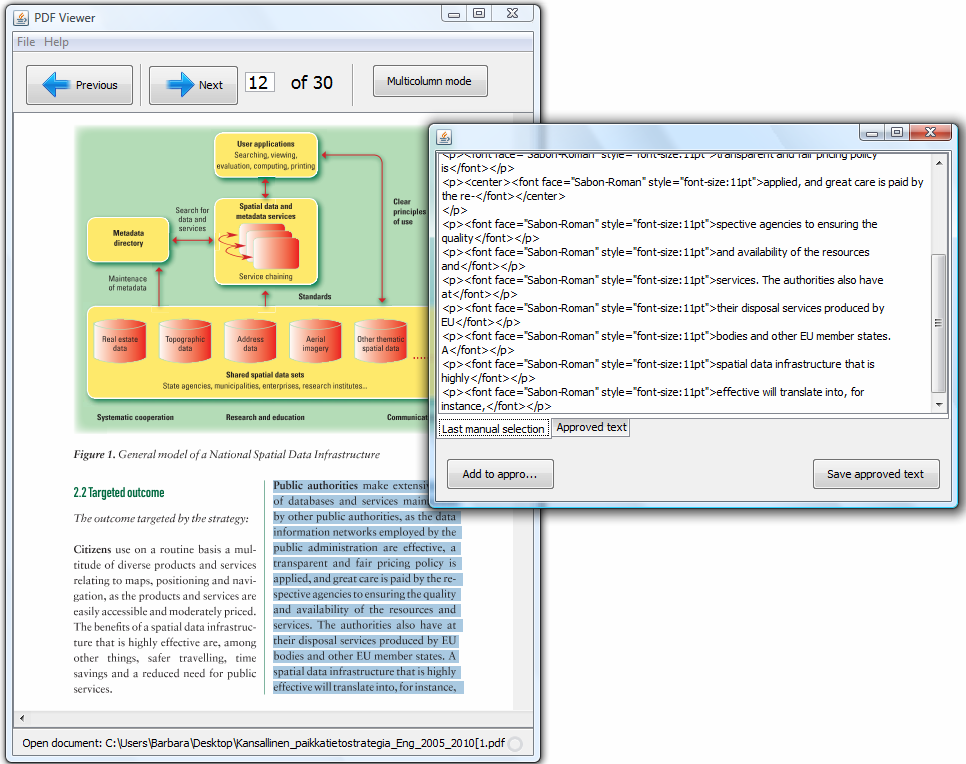
\includegraphics[width=\linewidth]{figures/book4all1.png}
	\caption{A view of the ad-hoc PDF Viewer extracting text from a multi-column layout document \protect\cite{book4all}}
	\label{fig:book4all1}
\end{figure}

Book4All attempts to semi-automate the conversion process as far as possible, but still offers the option of post processing the resulting markup as shown in figure~\ref{fig:book4all1}. While this is optional, important parts like alternative text for images can only be added like this. The markup is in Intermediate Book Format (IBF), which is based on XML. Without basic knowledge of XML, post-processing becomes much more difficult. 

\begin{figure}[H]
	\centering
	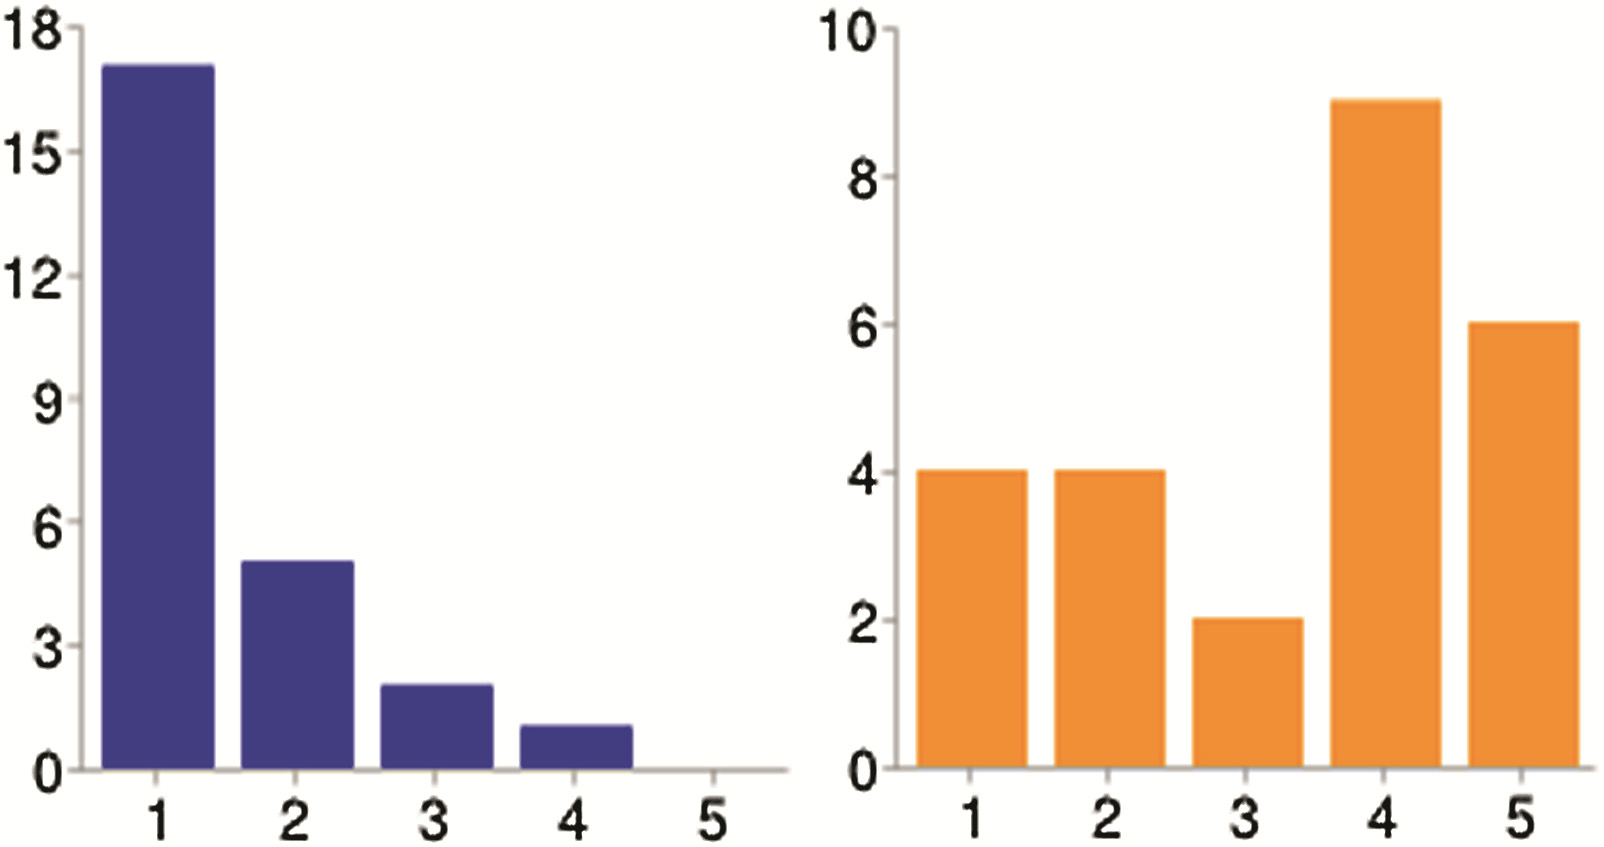
\includegraphics[width=\linewidth*4/5]{figures/easeOfContentAccess.png}
	\caption{Difficulty degree to access the content for the EPUB (blue, left) and PDF (orange, right), respectively (1-not difficult
		to 5-very difficult) \protect\cite{enrichEPUB}} 
	\label{fig:enrichEpub1}
\end{figure}

Bartalesi and Leporini \cite{enrichEPUB} also carried out an online survey in a follow-up work and asked 25 users to rate "enriched" EPUBs created in Book4All in comparison to the original PDF format regarding accessibility and usability. $50\%$ of respondents preferred EPUB over other e-book formats, while $13\%$ said EPUB was equivalent.
The sample group also felt that it was easier to access content in EPUBs and use the table of contents than in PDFs.
Furthermore, $80\%$ of blind users were unable to read images in PDFs correctly with their screen reader, while the corresponding value for EPUBs was less than $50\%$. $64\%$ of users found the EPUB's document structure easy to understand. Users also reported that it is much easier to access content in the EPUB than in a PDF, as shown in figure~\ref{fig:enrichEpub1}.  The results show that EPUB is suitable format for blind people, if the EPUB contains proper tagging. 
Those works motivate us to develop a new universal approach.

  % Grundlagen
%% analyse.tex
%% $Id: analyse.tex 28 2007-01-18 16:31:32Z bless $

\chapter{Analysis}
\label{ch:Analysis}


     % Analyse
%% entwurf.tex
%% $Id: entwurf.tex 28 2007-01-18 16:31:32Z bless $
%%
%% ==============================
\chapter{Design}
\label{ch:Design}


     % Entwurf
\chapter{Implementation of your Project}
\label{ch:Implementation}    % Implementierung
%% eval.tex
%% $Id: eval.tex 5 2005-10-10 20:55:48Z bless $

%%%%%%%%%%%%%
\chapter{Evaluation}
\label{ch:Evaluation}
%%%%%%%%%%%%%
        % Evaluierung
%% zusammenf.tex
%% $Id: zusammenf.tex 4 2005-10-10 20:51:21Z bless $
%%

\chapter{Future Work}
\label{ch:FutureWork}
%% ==============================
%
The Accessible EPUB editor is in a functional state where accessible EPUBs of the both new document standards, CSS and JavaScript can be created and edited. However, there is still much to be done.

The JavaScript document standard supports multiple HTML files as content documents. If the reading system supports local or session storage, it remembers which display style is to be displayed across several HTML files. This is actually the case with JavaScript standard in its current state as the first page with version switching mechanism is on a different page from the actual content. Accessible EPUB does not yet support multiple content pages. One issue mentioned in chapter \ref{ch:AccessibleEPUB Editor} is there are issues with long documents. The preview browser automatically scrolls to the top as soon as the user writes something in the editor. If Accessible EPUB allows the user to add another content page, this problem can be avoided. Furthermore, the user can create documents with several sections and these can be managed individually. This does not work with the CSS standard as CSS changes are local to a HTML file and do not persist across multiple of them.

Future development will focus on usability and simplified import of other document standards. Allowing users to import files of different formats will allow an easier transition to Accessible EPUB. The features will be implemented for two formats at first: text documents and HTML files. Importing text documents is quite simple as the file just has to be read and the contents have to be inserting into the editor. Importing HTML files is a bit more complicated. Instead of inserting into the editor, the back end web browser of the editor must be inserted to. Images and equations will not be in the form of the accessible EPUB document standard, so they have to be converted into the correct form. The program will present the user with a process to examine every image and equation and insert alternative text when necessary. Other formats can be imported with the tool pandoc converting them. It is already a part of Accessible EPUB so it does not require any additional programs.

Another feature advanced users may want is a source code editor. As mentioned in chapter \ref{ch:AccessibleEPUB Editor} a code viewer is already available, but it currently displays the entire file with the inner workings. It is also disabled as there were several issues with it. If a code editor is included, the user should not be able to see the inner workings of the document standard, since editing those might break the EPUB file and make it unreadable. 

\begin{comment}
\begin{figure}
	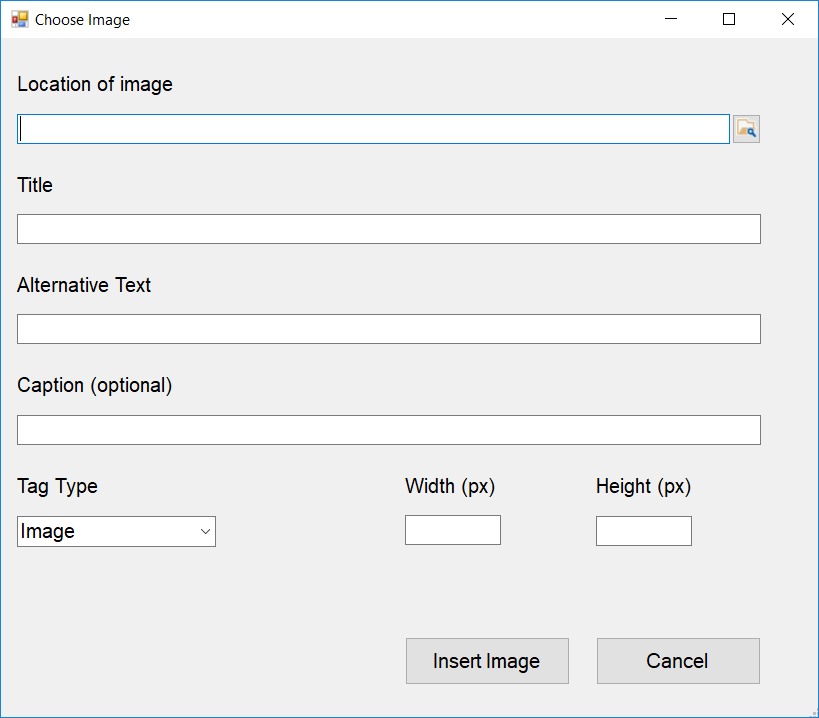
\includegraphics[width=\linewidth]{figures/imageDialogBox.png}	
	\caption{Insert image window of Accessible EPUB}
	\label{fig:imageDialogBox1}
\end{figure}
\end{comment}

To improve accessibility for visually impaired users, it should be possible to add an alternative image which can be a high contrast version of the original image. In addition to the one image document creators have to add, there will be an option to another one. This image will only be shown in the visually impaired display style. If no secondary image was chosen, the regular image will be displayed instead.

Training material has to be prepared so that users can get to know the EPUB standard and Accessible EPUB, like workshops which will users to test the standard and program. There will also be step-by-step tutorials to guide people through the document creation process and how to use all tools in the program.


\begin{comment}
There is still some room for improvement in the compatibility of the EPUB standard, so that it will also be possible to use the documents better with "older" EPUB readers. 
The JavaScript document standard supports multiple HTML files as content documents. If the reader system supports local or session storage, it remembers which version is to be displayed across several HTML files. Accessible EPUB does not yet support this. Adding this feature would allow users to create longer documents and manage individual sections.

Future development will focus on usability and simplified import of other document standards. Currently, users can already import text and HTML documents with certain restrictions so that they can keep their work in these formats. The tool PANDOC can serve as a basis for many formats.
Furthermore, images and formulas will not yet be in the format specified by the document standard during an import, so a wizard will be added that works through each image and formula and allows the user to enter alternative texts.  

Another feature advanced users may want is a source code editor. A code viewer is already available, but currently displays the entire file with the inner workings. The user should not be able to see it, since the processing increases the error possibilities in the document.

We are also considering whether we will start developing suitable readers for various end devices.
\end{comment}

\chapter{Conclusion}
\label{ch:Conclusion}

A short introduction is given where the motivation of this project and a short overview of the file format EPUB is presented. An EPUB document standard has been developed to allow visually impaired, blind and normal-sighted users to use the same document while meeting their respective accessibility requirements. There are two different versions of it, one using JavaScript and the other using CSS. Both versions of the document standard were tested on several reading systems. Only very few of the reading systems were able to show MathML equations and even fewer were able to display the document standards properly. 

EPUB 3 is not widely supported by reading systems. The switching mechanism only worked on four out of fourteen. MathML rendered on nine of them, and many reading systems were chosen because they supported it. Developers still have a lot of work to do for EPUB 3 to have support in their reading systems.

An editor called "Accessible EPUB" was created so that users without programming knowledge can create accessible documents. It allows the user to write text much like in an word processor and insert mathematical equations, images and tables. The document standard uses EPUB 3, which is not yet fully supported by most EPUB reading systems. It is planned to add features to improve the usability of Accessible EPUB, such as importing files of different formats and further tools for accessibility.
  % Future Work
\include{summary}   % Zusammenfassung und Ausblick

%% ++++++++++++++++++++++++++++++++++++++++++
%% Anhang
%% ++++++++++++++++++++++++++++++++++++++++++

\appendix
%\include{anhang_a}
%\include{anhang_b}

%% ++++++++++++++++++++++++++++++++++++++++++
%% Literatur
%% ++++++++++++++++++++++++++++++++++++++++++
%  mit dem Befehl \nocite werden auch nicht 
%  zitierte Referenzen abgedruckt
\cleardoublepage
\phantomsection
\addcontentsline{toc}{chapter}{\bibname}
%%
%\nocite{*} % nur angeben, wenn auch nicht im Text zitierte Quellen 
           % erscheinen sollen
%\bibliographystyle{itmabbrv} % mit abgekürzten Vornamen der Autoren
%\bibliographystyle{gerplain} % abbrvnat unsrtnat
% spezielle Zitierstile: Labels mit vier Buchstaben und Jahreszahl
%\bibliographystyle{itmalpha}  % ausgeschriebene Vornamen der Autoren
\printbibliography
%% ++++++++++++++++++++++++++++++++++++++++++
%% Index
%% ++++++++++++++++++++++++++++++++++++++++++
\ifnotdraft{
\cleardoublepage
\phantomsection
\printindex            % Index, Stichwortverzeichnis
}
\end{document}
%% end of file

